\normalfalse \difficiletrue \tdifficilefalse
\correctionfalse

%\UPSTIidClasse{11} % 11 sup, 12 spé
%\newcommand{\UPSTIidClasse}{11}

\exer{Mouvement RR 3D  $\star\star$ \label{C2:09:08}}
\setcounter{question}{0}\UPSTIcompetence[2]{C2-09}
\index{Compétence C2-09}
\index{Principe fondamental de la dynamique}
\index{PFD}
\index{Mécanisme à 2 rotations 3D}
\ifcorrection
\else
\textbf{Pas de corrigé pour cet exercice.}
\fi

\ifprof
\else
Soit le mécanisme suivant. On a $\vect{AB}=H\vect{j_1}+R\vect{i_1}$ et $\vect{BC}=L\vect{i_2}$. On a $H=\SI{20}{mm}$, $r=\SI{5}{mm}$, $L=\SI{10}{mm}$. De plus :
\begin{itemize}
\item $G_1$ désigne le centre d'inertie de \textbf{1} tel que $\vect{AG_1}=H\vect{j_1}$, on note $m_1$ la masse de \textbf{1} et $\inertie{G_1}{1}=\matinertie{A_1}{B_1}{C_1}{0}{0}{0}{\bas{1}}$; 
\item $G_2=C$ désigne le centre d'inertie de \textbf{2}, on note $m_2$ la masse de \textbf{2} et $\inertie{G_2}{2}=\matinertie{A_2}{B_2}{C_2}{0}{0}{0}{\bas{2}}$.
\end{itemize}

Un moteur électrique positionné entre \textbf{0} et \textbf{1} permet d'actionner le solide \textbf{1}.
Un moteur électrique positionné entre \textbf{1} et \textbf{2} permet d'actionner le solide \textbf{2}.
L'accélération de la pesanteur est donnée par $\vect{g}=-g\vect{j_0}$.

\begin{center}
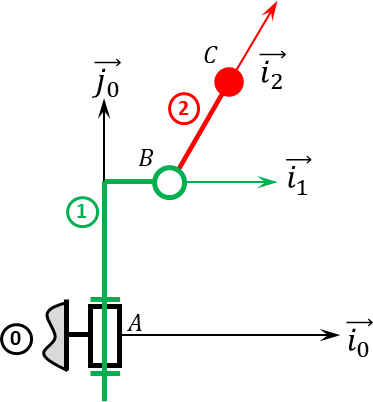
\includegraphics[width=\linewidth]{08_RR3D_01}
\end{center}
\fi

\question{Dans le but d'obtenir les lois de mouvement, appliquer le théorème du moment dynamique au solide \textbf{2} au point $B$ en projection sur $\vect{k_1}$ puis le théorème du moment dynamique à l'ensemble \textbf{1+2} au point $A$ en projection sur $\vect{j_0}$}
\ifprof
\else
\fi

\ifprof
\else
\begin{flushright}
\footnotesize{Corrigé  voir \ref{C2:09:08}.}
\end{flushright}%
\fi